% !TeX root = thesis_guide.tex
% chktex-file 1 chktex-file 21

%==============================================================================
\chapter{Figures and Feynman graphs}%
\label{sec:fig}\index{figures}\index{Feynman graph}
%==============================================================================

\LaTeX{} file: \url{./guide_figs.tex}\\[1ex]
\noindent
This chapter discusses what you need to know to include graphics in
your thesis. The basic command to use is \Macro{includegraphics}.

I found a pretty complete guide (in German) called \texttt{l2piqfaq}
which can be obtained from
\url{http://www.ctan.org/tex-archive/info/l2picfaq/german}. It contains
a lot of detailed information and tricks.

The chapter also contains some suggestions as to how to create Feynman
graphs with a number of different packages.

%------------------------------------------------------------------------------
\section{Simple figures}%
\label{sec:fig:simple}
%------------------------------------------------------------------------------

A simple figure and its associated caption is straightforward to
include. For example, the layout of the LHC and its experiments is
shown in \cref{fig:LHC}.

\begin{figure}[htbp]
  \centering
  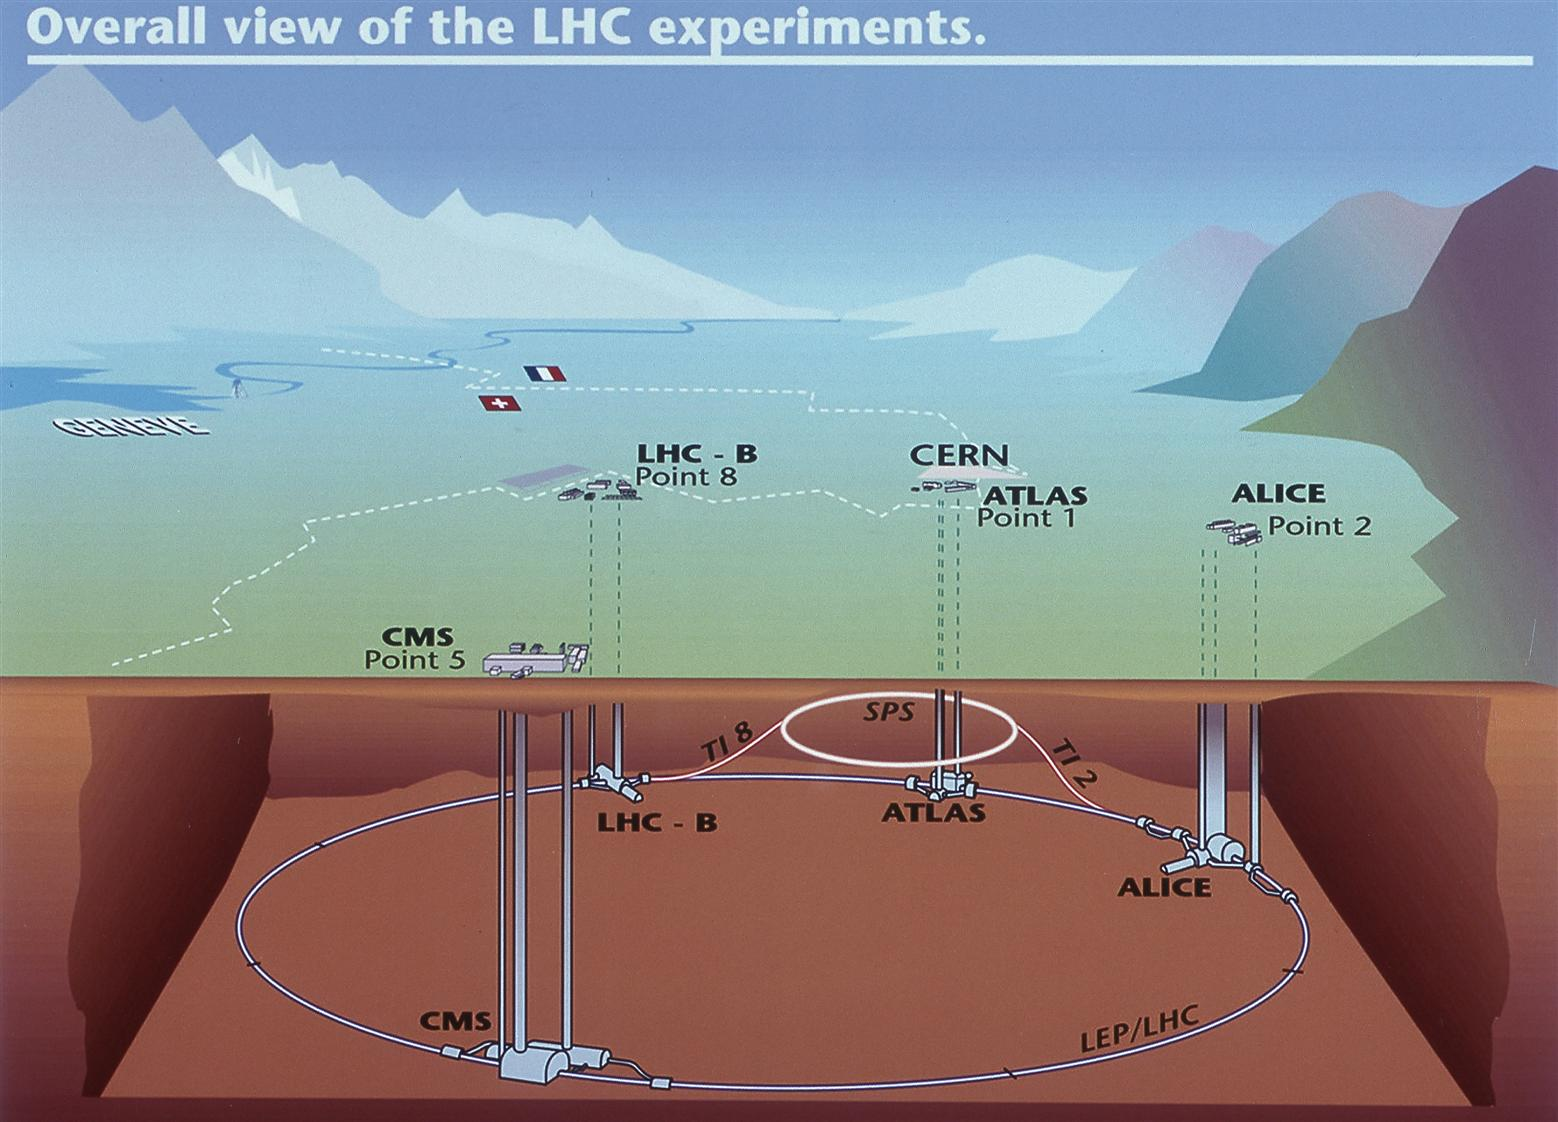
\includegraphics[width=\figwidth]{CERN_all-experiments}
  \caption[Sketch of the LHC ring, the position of the experiments and
  the surrounding countryside.]{Sketch of the LHC ring, the position
    of the experiments and the surrounding countryside. The four big
    LHC experiments are indicated. The location of the injection lines
    and the SPS are also shown.}%
  \label{fig:LHC}
\end{figure}

Note the use of \Macro{centering} rather than the environment
\BegEnv{center} \ldots \EndEnv{center} to centre the figure. This
avoid adding extra vertical space. It is also important that the
\Macro{label} be either inside the caption or after it. If your
caption is more than 1 (or 2) lines, you should also give a short form
that will appear in the ``List of Figures''.

One tricky question is how to best format the caption. This document
uses a smaller font and no extra indentation. Often italics are
used. I dislike this, as symbols are then formatted in different ways
in the main text and in the caption. One can also reduce the width of
the caption. The font for the caption can be specified using the
\Macro{setkomafont}\texttt{\{caption\}} command. You can specify how
to label the figure by changing the \Macro{figureformat} command. The
captions in this document follow the standard \KOMAScript{}
convention: if they are one line long they are centred; if they are
longer they are left-adjusted. If you want them all to be
left-adjusted set the \Option{KOMAoptions} \Option{caption=nooneline}
in \texttt{ubonn-thesis.sty}. Some examples of the possibilities are
included in the style file.

Another thing to consider is whether the text should be indented or
not. For short captions, indentation is OK\@. I do not think it looks
good for long captions. Hence the style file sets
\Macro{setcapindent}\texttt{\{0pt\}}.

%------------------------------------------------------------------------------
\section{Fancier figures}%
\label{sec:fig:fancy}\index{figures!multiple}
%------------------------------------------------------------------------------

Life gets more complicated if you want to include several plots in
one figure, if you want the caption next to the figure, or if you want
the text to \enquote{flow} around the figure. For the first case I like to
use the \Env{tabular} environment to place the plots, although
there are other ways of doing it.

Another very nice way to add (a), (b) etc.\ to the figure is to use the
\Macro{put} command. This has the big advantage that you can display
the letters in the figure without actually having to add them to the
EPS/PDF file. \Cref{fig:letters1} shows how this is done. Note
that the origin of the coordinate system is the bottom right-hand
corner of the file that you have included (assuming that the
\Macro{put} command comes just after the \Macro{includegraphics}).
The units for the \Macro{put} command are set with the
\Macro{setlength}\texttt{\{\textbackslash unitlength\}} command, which
is by default set to \SI{1}{\mm} in \texttt{ubonn-thesis.sty}.
The same units are also used for Feynman graphs made with the
\Package{feynmf} and/or \Package{feynmp} package --- see
\cref{sec:fig:feynman:feynmp}.

\begin{figure}[htbp]
  \centering
  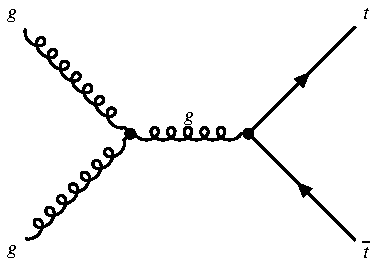
\includegraphics[height=3cm]{gg_ttbar_1-BW}\quad
  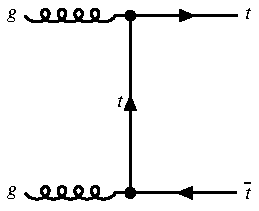
\includegraphics[height=3cm]{gg_ttbar_2-BW}\quad
  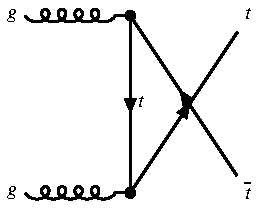
\includegraphics[height=3cm]{gg_ttbar_3-BW}
  \put(-130,14){(a)}
  \put(-80,14){(b)}
  \put(-35,14){(c)}
  \caption{Adding letters to figures with \Macro{put}.}%
  \label{fig:letters1}
\end{figure}

Another way of achieving the same thing, but this time with the letter
outside the figure is to use \Env{tabular}. An example of this is
shown in \cref{fig:letters2}.

\begin{figure}[htbp]
  \centering
  \begin{tabular}{ccc}%@{\hspace*{0.15\figwidth}}p{0.33\figwidth}p{0.33\figwidth}l}
    % \multicolumn{3}{c}{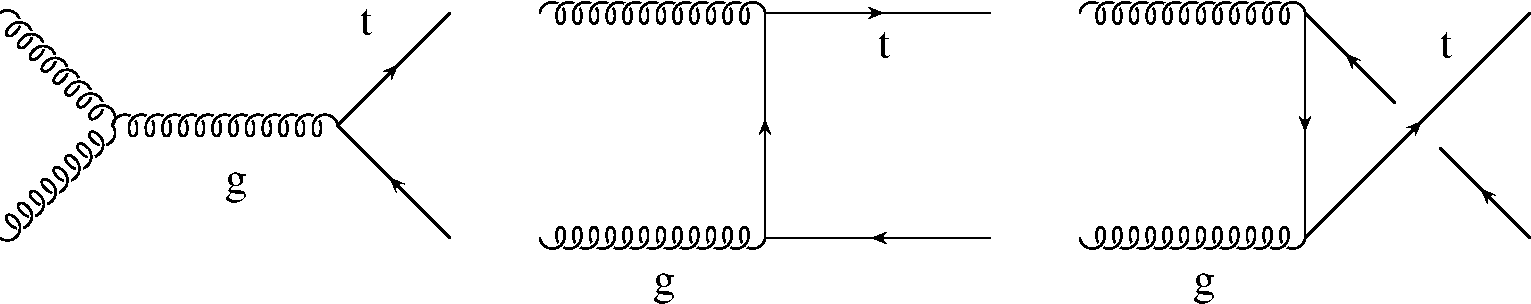
\includegraphics[width=\figwidth]{gg_tt}}\\
    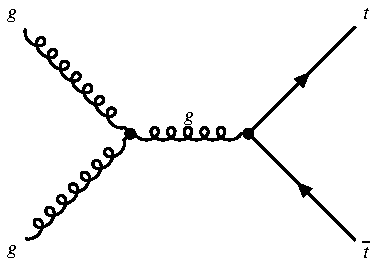
\includegraphics[width=0.33\figwidth]{gg_ttbar_1-BW} &
    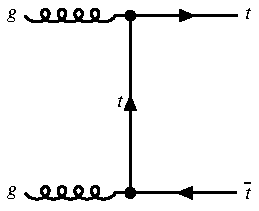
\includegraphics[width=0.3\figwidth]{gg_ttbar_2-BW} &
    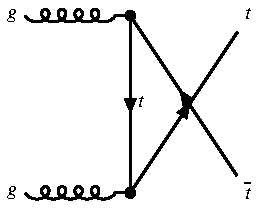
\includegraphics[width=0.3\figwidth]{gg_ttbar_3-BW}\\
    (a) & (b) & (c)
  \end{tabular}
  \caption{Adding letters to figures with \Env{tabular}.}%
  \label{fig:letters2}
\end{figure}

If you want to save space it is sometimes nice to put the caption next
to the figure. While packages exist to do this, \KOMAScript{} has its
own built-in \Env{captionbeside} environment. The placement option comes
after the caption itself and can be one of:
\begin{description}\setlength{\parskip}{0pt}
\item[l] Left of figure
\item[r] Right of figure
\item[i] Inner margin in two-sided layout
\item[o] Outer margin in two-sided layout
\end{description}
Note that this is an environment rather than a macro and that the
figure itself is inside the environment. Also the placement does not
seem to work exactly how it is advertised in the manual. I set the
width equal to \Macro{figwidth} and then the offset to \texttt{-\Macro*{figwidth}}.

\begin{figure}[htbp]
  \centering
  \begin{captionbeside}{A small figure with a simple caption beside it.}[i][\figwidth][-\figwidth]
    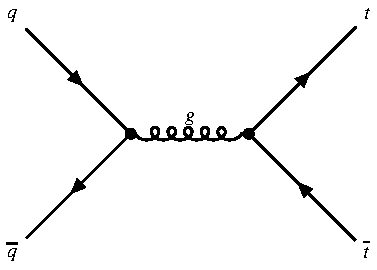
\includegraphics[width=0.3\textwidth]{qq_ttbar-BW}
  \end{captionbeside}%
  \label{fig:qqtt}
\end{figure}

If you want different (partial) captions for a figure then the
\Package{subfig} package used to be the way to go. 
An alternative, and successor, to \Package{subfig} is
\Package{subcaption}. It works in much the same way as
\Package{subfig}. A nice tutorial on its use can be found in
\url{http://www.peteryu.ca/tutorials/publishing/latex_captions}.
An example of its use can be seen in \cref{fig:nccc}.
The \LaTeX\ file \texttt{guide\_figs.tex} contains examples for both \Package{subfig} and 
\Package{subcaption}.
% , as the way \Package{subcaption} should be used was different for \TeXLive 2011 and earlier.
You can see how to reference
the different parts of the figure in \cref{sec:fig:feynman}. If
you want the captions of the sub-figures to also appear in the
\enquote{List of Figures} you should include the package with the
option \Option{lofdepth}. For tables use the option \Option{lotdepth}.


% \ifthenelse{\texlive < 2012}{%
% \begin{figure}[htbp]
%   \centering
%   \subfloat[NC scattering]{%
%     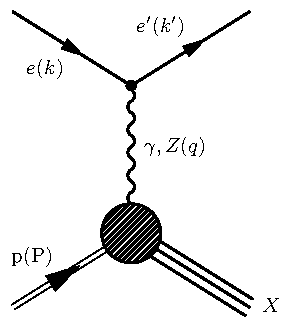
\includegraphics[width=0.5\figwidth]{ep_nc}%
%     \label{fig:nccc-nc}
%   }
%   \qquad
%   \subfloat[CC scattering]{%
%     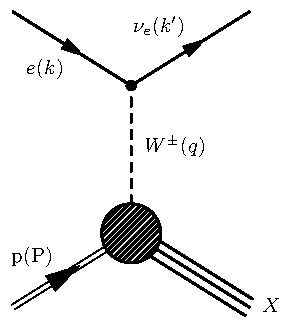
\includegraphics[width=0.5\figwidth]{ep_cc}%
%     \label{fig:nccc-cc}
%   }
%   \caption{Processes in $ep$ scattering.}%
%   \label{fig:nccc}
% \end{figure}
% }{%
\begin{figure}[htbp]
  \centering
  \begin{subfigure}[b]{0.5\figwidth}
    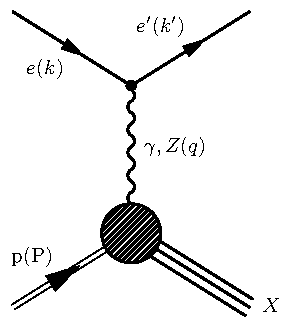
\includegraphics[width=0.5\figwidth]{ep_nc}
    \caption{NC scattering}\label{fig:nccc-nc}
  \end{subfigure}
  \qquad
  \begin{subfigure}[b]{0.5\figwidth}
    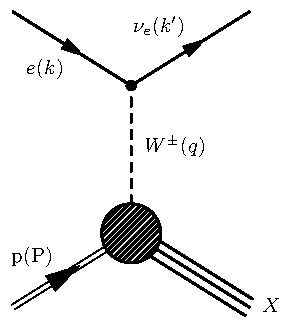
\includegraphics[width=0.5\figwidth]{ep_cc}
    \caption{CC scattering}\label{fig:nccc-cc}
  \end{subfigure}
  \caption{Processes in $ep$ scattering.}%
  \label{fig:nccc}
\end{figure}
% }

If you run out of space (applies more often to proceedings than to
theses) you can use the \Package{wrapfig} package.


%------------------------------------------------------------------------------
\section{Figure formats}%
\label{sec:fig:formats}\index{figures~formats}
%------------------------------------------------------------------------------

If you use plain \LaTeX, you are pretty much stuck with encapsulated
postscript (EPS) as your figure format. If you use pdf\LaTeX, then you
have much more freedom, with the notable exception that you cannot
include EPS files!\footnote{%
This restriction has finally been lifted with \TeXLive 2011. It
simply converts the EPS files to PDF inline.}
I would still recommend that you always try to use
a vector graphic format. What usually works well is to either create
PDF directly or to create EPS and then convert from EPS to PDF\@.

The tool I use for conversion is \texttt{epstopdf}. Occasionally this
fails; in that case \texttt{eps2eps} can help. It is important that
the bounding box is set correctly in the EPS file before you run
\texttt{epstopdf}.

If these fail, you can try the \texttt{convert} command which is part
of \texttt{ImageMagick}. A more powerful tool is \texttt{inkscape}
which is a successor to \texttt{xfig}. Professionals use Adobe Illustrator!


%------------------------------------------------------------------------------
\section{Placement}%
\label{sec:fig:placement}
%------------------------------------------------------------------------------

Even after many years of including figures into \LaTeX{} files, I
still think there is a fair amount of black magic involved in getting
them into the place that you want them to be.

In general, you are advised to give \LaTeX{} as much freedom as
possible in the placing, so it is usual to use the options
\Option{[htbp]} for the placement.
In particular, be very careful with
using just \Option{[h]} or \Option{[H]} as the placement option. It very
easily leads to \LaTeX{} putting single lines of text either above or
below a figure.
One way to get rid of single lines is to remove the option \Option{h},
as the figure must then be placed at the top or bottom of the page
(or on a page of floats).
You can also add an \Option{!} in the list
of options, which suspends spacing and number restrictions.

A nice summary of the logic behind the placement can be found in
\href{http://tex.stackexchange.com/questions/39017/how-to-influence-the-position-of-float-environments-like-figure-and-table-in-lat}{\TeX/\LaTeX\ Stack Exchange} (click on the link!).
A couple of points from there that are worth mentioning here:
\begin{itemize}
\item The order of the options \Option{htbp} has no effect!
\item If a float is placed in the middle of a paragraph,
  the reference point for deciding where it will appear is the next line break or page break in the paragraph,
  following the float.
\item The order of figures (and tables) is fixed to the order that they are included in a document.
  However, the order of figures and tables relative to each other is not fixed.
\end{itemize}

The
\href{http://www.tex.ac.uk/cgi-bin/texfaq2html?label=floats}{UK List of FAQ}
recommends changing several default \LaTeX\ options so that there are fewer problems
with figure and table placement.
It is certainly worth reading that page for further advice.
As it is very hard to really test how well these options work
they can be turned on or off in \Package{ubonn-thesis} via the option \Option{floatopt=true|false}.
The default value is set to \Option{true}.

I used to think it was better to attach the figure to a paragraph.
More recently it appears to me to be better to separate the figure
from the paragraph.
What I mean is illustrated below:
\begin{tcblisting}{listing only}
\Cref{fig:funny1} is attached to the paragraph.
%
\begin{figure}[htbp]
  \centering
  \includegraphics[width=\figwidth]{file}
  \caption{An odd plot that I don't understand.}
  \label{fig:funny1}
\end{figure}
%
The distribution shows something that I do not understand.

Given that this is not understood we went to the pub for a beer to
think about it a bit more.
\end{tcblisting}

\begin{tcblisting}{listing only}
\Cref{fig:funny2} is separated from the paragraph by a blank line.
The distribution shows something that I do not understand.

\begin{figure}[htbp]
  \centering
  \includegraphics[width=\figwidth]{file}
  \caption{An odd plot that I don't understand.}
  \label{fig:funny2}
\end{figure}

Given that this is not understood we went to the pub for a beer to
think about it a bit more.
\end{tcblisting}

However, it is hard to give a hard and fast rule here.
As indicated above, the effect of these different ways of including a figure (and table) is the point in the text (reference point) that \LaTeX\ uses to start trying to place the figure.
In general, you should only try to tweak the position of figures and tables when your text is final,
as a change in the text way well move some of the floats.

%------------------------------------------------------------------------------
\subsection{\Package{standalone} package and class}%
\label{sec:fig:standalone}

The \Package{standalone} package provides a great way of developing
figures in small files and then inputting these files directly,
without making any changes, into your thesis!

It is in fact both a package and a document class. It is
available from \TeXLive 2012 onward. It allows you to have a
standalone document for a \Package{\TikZ} or \Package{feynmf} figure
and also input this file into another document. If you run pdf\LaTeX\
on the file it also automatically crops the resulting picture. This is
one of those packages where you think
\enquote{Why didn't someone create this years ago?}.
The \TikZ figures (as well as those made using \Package{TikZ-FeynHand})
that I include in this guide (see subdirectories \texttt{tikz} and \texttt{pyfeynhand})
make use of this package.
If you want to use it, make sure that you also include this package in
your thesis.


%------------------------------------------------------------------------------
\section{Feynman graphs}%
\label{sec:fig:feynman}\index{figures!Feynman graphs}\index{Feynman graphs}
%------------------------------------------------------------------------------

You have lots of Feynman graphs you want to include, but how do you
generate them? 
For a few years I used a Python package \Package{PyFeyn} (\url{https://pyfeyn.hepforge.org})
that works quite nicely once you have it set up.
However, the package does not seem to be actively developed any more
and fixes are needed before it works with the latest \Package{PyX} version,
which is the drawing tool it uses.
Hence, I am moving my graphs to a \TikZ package, which means that they are created in a \LaTeX\ file.
Two possibilities are \Package{TikZ-Feynman} and \Package{TikZ-FeynHand}.
I have written a Python wrapper for \Package{TikZ-FeynHand},
which hopefully allows me to combine the best of both worlds!
The wrapper code and an example can be found in the \File{pyfeynhand} directory.

Before I started using Python packages, I followed the example of many people,
where I found one way doing making graphs and never changed!
I used \texttt{Mn\_Fit},
mainly because I wrote it and therefore know inside out how it works.
Examples can be found on my web page:
\url{http://pi.physik.uni-bonn.de/~brock/feynman}.
Alternatives include \Package{axodraw} and the \Package{feynmf} or
\Package{feynmp} packages.

The use of \Package{feynmf} and \Package{feynmp} is
described in \cref{sec:fig:feynman:feynmp}, while a few
examples of usage of \Package{\TikZ} are given in
\cref{sec:fig:feynman:tikz}.
Usage of \Package{TikZ-FeynHand} and my Python wrapper \Package{PyFeynhand}
can also be found in \cref{sec:fig:feynman:tikz}.
Examples of Feynman graphs made
with \Package{feynmf} and \Package{feynmp} can be found in the \texttt{feynmf} directory;
those made with \Package{TikZ-FeynHand} can be found in the \texttt{pyfeynhand} and \texttt{tikz} subdirectories;
while those made with \Package{\TikZ} can be found in the \texttt{tikz} subdirectory.

Instructions on how to use \Package{axodraw} may come at a later
date --- contributions would be welcome! Several people have claimed
that \texttt{jaxodraw} is the way to go. This is a Java package which
you can download from \url{http://jaxodraw.sourceforge.net/}. It has
a Graphical User Interface (GUI) to \Package{axodraw} and so is simple and
straightforward to use.

This paragraph illustrates how to reference different parts of a
figure that uses the environment \Env{subfigure} from the package \Package{subcaption}.
If you compile the guide with \TeXLive 2011 or earlier the
environment \Env{subcaption} from the package \Package{subfig} is used.
The NC and CC graphs shown in
\cref{fig:nccc}, or more accurately in \cref{fig:nccc-nc} and
\cref{fig:nccc-cc} were made with \Package{feynmp}. Another way of
saying the same thing is that typical Feynman graphs for \(ep\)
scattering are shown in \cref{fig:nccc}, where
\subref{fig:nccc-nc} shows a neutral current and \subref{fig:nccc-cc}
show a charged current process.


%------------------------------------------------------------------------------
\subsection{Feynman graphs with \TikZ}%
\label{sec:fig:feynman:tikz}\index{TikZ@\TikZ}

There are (at least) two packages based on \TikZ that exist to draw Feynman graphs:
\Package{TikZ-Feynman} and \Package{TikZ-FeynHand}.
If you want to use the automatic placement features of \Package{TikZ-Feynman}
you have to use \LuaLaTeX.
Hence, I am inclined to use the \Package{TikZ-FeynHand} package.\footnote{%
Note that the \Package{TikZ-FeynHand} package was first included in \TeXLive 2017.}
It does not seem to be possible to adjust the amplitude and frequency
of boson and gluon oscillations explicitly.
This has to be done using the \Macro*{setlength\{\textbackslash feynhandlinesize\{1.0pt\}\}} command.
This also, as the name suggest, changes the line thickness.
After a bit of playing around \num{1.0}{pt} seems to work well,
with a Feynman graph size of about \SI[parse-numbers=false]{2 \times 2}{\cm^{2}}

I like using a scripting language, e.g.\ Python, to draw my graphs.
I have therefore written a Python wrapper for \Package{TikZ-FeynHand}.
You can find the wrapper and an example script in the \File{pyfeynhand} directory.
The wrapper creates a \LaTeX{} file,
which can either be compiled or included directly in your document,
as it uses the \Package{standalone} package.

\Cref{fig:feyn:tdecay} shows two graphs from one of my favourite processes.
These graphs are made using \Package{TikZ-FeynHand} commands directly,
while the \TeX{} file was created using the Python wrapper.

\begin{figure}[htbp]
  \centering
  \begin{subfigure}{0.5\figwidth}
    \centering
    \ifthenelse{\texlive > 2016}{%
      \documentclass{standalone}
\usepackage[utf8]{inputenc}
\usepackage{newtxtext}
\usepackage{newtxmath}
\usepackage[italic]{hepnicenames}
\makeatletter\def\@shiftlen@anti@gen@bar{0mu}\makeatother
\usepackage[svgnames]{xcolor}
\usepackage{tikz-feynhand}


\begin{document}
\begin{tikzpicture}
  \setlength{\feynhandlinesize}{1.0pt}
  \tikzfeynhandset{every dot={/tikz/color=Crimson},}
  \begin{feynhand}
    \vertex [particle, Blue] (t) at (-3.0, 1.0) {\Ptop};
    \vertex [particle, IndianRed] (b) at (3.0, 0.0) {\Pbottom};
    \vertex [particle, DarkCyan] (l) at (3.0, 2.0) {\color{DarkCyan}\Plepton};
    \vertex [particle, DarkCyan] (nu) at (3.0, 4.0) {\color{DarkCyan}\APnulepton};
    \vertex [dot, Crimson] (tb) at (-0.5, 1.0) {};
    \vertex [dot, Crimson] (Wlnu) at (1.0, 3.0) {};
    \propagator [fermion, Blue] (t) to (tb);
    \propagator [fermion, IndianRed] (tb) to (b);
    \propagator [boson, ForestGreen] (tb) to [edge label=\PW, color=ForestGreen] (Wlnu);
    \propagator [fermion, DarkCyan] (Wlnu) to (l);
    \propagator [fermion, DarkCyan] (nu) to (Wlnu);
  \end{feynhand}
\end{tikzpicture}
\end{document}

    }{%
      \missingfigure{TeX Live version does not include TikZ-FeynHand}
    }
    \caption{\LaTeX\ file}%
    \label{fig:feyn:tdecay1}
  \end{subfigure}
  \qquad
  \begin{subfigure}{0.5\figwidth}
    \centering
    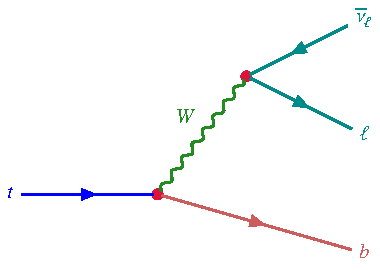
\includegraphics[width=0.5\figwidth]{../tikz/tdecay}
    \caption{PDF file}%
    \label{fig:feyn:tdecay2}
  \end{subfigure}
  \caption{Feynman graphs made with the \Package{TikZ-FeynHand} package.
    This example uses the \Env{subfigure} environment from the \Package{subcaption} package.}%
  \label{fig:feyn:tdecay}
\end{figure}

A diagram for \Pgm decay using the \Package{TikZ-Feynman} package
is shown in \cref{fig:feyn:mudecay}.
This uses the manual placement style so that I can compile the guide with an \TeX\ engine.

\begin{figure}[htbp]
  \centering
  \begin{subfigure}{0.6\figwidth}
    \centering
    \documentclass{standalone}

\usepackage[utf8]{inputenc}
\usepackage{newtxtext}
\usepackage{newtxmath}
\usepackage[italic]{heppennames}
\usepackage[svgnames]{xcolor}
\usepackage{tikz-feynman}

\begin{document}
\begin{tikzpicture}
  \begin{feynman}
    \vertex (a) {\(\mu^{-}\)};
    \vertex [right=of a] (b);
    \vertex [above right=of b] (f1) {\(\nu_{\mu}\)};
    \vertex [below right=of b] (c);
    \vertex [above right=of c] (f2) {\(\overline \nu_{e}\)};
    \vertex [below right=of c] (f3) {\(e^{-}\)};

    \diagram* {
      (a) -- [fermion] (b) -- [fermion] (f1),
      (b) -- [boson, edge label'=\(W^{-}\)] (c),
      (c) -- [anti fermion] (f2),
      (c) -- [fermion] (f3),
    };
  \end{feynman}
\end{tikzpicture}
\end{document}
    \caption{\LaTeX\ file}%
    \label{fig:feyn:mudecay1}
  \end{subfigure}
  \qquad
  \begin{subfigure}{0.4\figwidth}
    \centering
    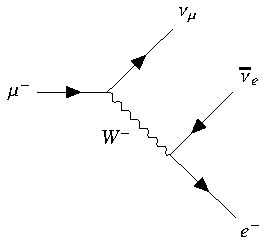
\includegraphics[width=0.4\figwidth]{../tikz/mudecay-feynman}
    \caption{PDF file}%
    \label{fig:feyn:mudecay2}
  \end{subfigure}
  \caption{Feynman graphs made with the \Package{TikZ-Feynman} package.
    This example uses the \Env{subfigure} environment from the \Package{subcaption} package.
    The example is taken from \url{https://www.overleaf.com/learn/latex/feynman_diagrams}.}%
  \label{fig:feyn:mudecay}
\end{figure}

If you want to draw Feynman graphs using \TikZ directly,
you need to include some extra \TikZ packages and libraries.
In addition it makes sense to
define things like gluons, photons and incoming and outgoing particles
once, as these are objects that are often needed.

% Given the multitude of possibilities that exist to draw things with
% \TikZ, it is not surprising that there are several ways of achieving the same end.
% If you want to work with \TikZ directly, you could also consider \Package{feymp},
% which has very similar capabilities and is dedicated to Feynman graphs.
% If you use \TikZ for drawing other things, then it is
% probably easier to use it also for Feynman graphs.
% However, if you want things like gluons on an arc, this may well only be available, if
% at all, with very recent versions of \Package{\TikZ}.

We can directly compare a scattering graph made with
\Package{feynmp}, \Package{\TikZ} and \Package{TikZ-FeynHand}.
This is shown in \cref{fig:feyn:cf}.
As you can see the quality of the graphs is very similar.
Further tweaking can probably make them almost identical.
In the \Package{TikZ-FeynHand} graph, I use lots of colours to illustrate how they work.

% \ifthenelse{\texlive < 2012}{%
% \begin{figure}[htbp]
%   \centering
%   \begin{minipage}[b]{0.5\figwidth}
%     \centering
%     \subfloat[Feynmp]{%
%       \begin{fmffile}{moeller}
  \begin{fmfgraph*}(40,30)
    \fmfleft{i1,i2}
    \fmflabel{$e^{-}$}{i1}
    \fmflabel{$e^{-}$}{i2}
    \fmfright{o1,o2}
    \fmflabel{$e^{-}$}{o1}
    \fmflabel{$e^{-}$}{o2}
    \fmf{fermion, fore=blue}{i1,v1,o1}
    \fmf{fermion, fore=blue}{i2,v2,o2}
    \fmf{photon,label=$\gamma$}{v1,v2}
    \fmfdot{v1,v2}
  \end{fmfgraph*}
\end{fmffile}

%       \ifthenelse {\texlive < 2011}{%
%       }{
%         \write18{mpost moeller}
%       }
%     }\label{fig:feyn:feynmp}
%   \end{minipage}
%   \qquad
%   \begin{minipage}[b]{0.5\figwidth}
%     \centering
%     \subfloat[\TikZ]{%
%       \ifthenelse {\texlive < 2011} {%
%         \fbox{\parbox[b]{0.4\textwidth}{%
%           Error messages appear when trying to
%           compile the guide with \Package{tikz} and \TeXLive 2009,
%           so the figure cannot be included.
%           See the file \texttt{../tikz/moeller.tex}.}}
%       }{%
%         \documentclass{standalone}

\usepackage{tikz}
\usepackage{tikz-3dplot}
\usepackage{pgfplots}
\usetikzlibrary{positioning,shapes,arrows}
\usetikzlibrary{decorations.pathmorphing}
\usetikzlibrary{decorations.markings}

\begin{document}
\tikzset{
  particle/.style={thick, draw=blue, postaction={decorate},
    decoration={markings, mark=at position 0.6 with {\arrow[blue]{triangle 45}}}},
  photon/.style={decorate, draw=black,
    decoration={coil, aspect=0}},
  gluon/.style={decorate, draw=black,
    decoration={coil, segment length=5pt, amplitude=4pt}}
}

\begin{tikzpicture}[node distance=1cm and 1.5cm]
  \coordinate[label=left:$e^{-}$] (e1);
  \coordinate[below right=of e1] (aux1);
  \coordinate[above right=of aux1,label=right:$e^{-}$] (e2);
  \coordinate[below=1.25cm of aux1] (aux2);
  \coordinate[below left=of aux2,label=left:$e^{-}$] (e3);
  \coordinate[below right=of aux2,label=right:$e^{-}$] (e4);

  \draw[particle] (e1)   -- (aux1);
  \draw[particle] (aux1) -- (e2);
  \draw[particle] (e3)   -- (aux2);
  \draw[particle] (aux2) -- (e4);
  \draw[photon]   (aux1) -- node[label=right:$\gamma$] {} (aux2);
\end{tikzpicture}
\end{document}

%       }
%     }\label{fig:feyn:tikz}
%   \end{minipage}
%   \caption{Feynman graphs drawn with \Package{feynmp} and \Package{tikz}.}%
%   \label{fig:feyn:cf}
% \end{figure}
% }{%
\begin{figure}[htbp]
  \centering
  \subcaptionbox{feynmp\label{fig:feyn:feynmp}}
    [0.3\textwidth]{\fbox{%
      \begin{fmffile}{moeller}
  \begin{fmfgraph*}(40,30)
    \fmfleft{i1,i2}
    \fmflabel{$e^{-}$}{i1}
    \fmflabel{$e^{-}$}{i2}
    \fmfright{o1,o2}
    \fmflabel{$e^{-}$}{o1}
    \fmflabel{$e^{-}$}{o2}
    \fmf{fermion, fore=blue}{i1,v1,o1}
    \fmf{fermion, fore=blue}{i2,v2,o2}
    \fmf{photon,label=$\gamma$}{v1,v2}
    \fmfdot{v1,v2}
  \end{fmfgraph*}
\end{fmffile}

      \write18{mpost moeller}}
  }
  \subcaptionbox{\TikZ\label{fig:feyn:tikz}}
    [0.3\textwidth]{\fbox{%
    \documentclass{standalone}

\usepackage{tikz}
\usepackage{tikz-3dplot}
\usepackage{pgfplots}
\usetikzlibrary{positioning,shapes,arrows}
\usetikzlibrary{decorations.pathmorphing}
\usetikzlibrary{decorations.markings}

\begin{document}
\tikzset{
  particle/.style={thick, draw=blue, postaction={decorate},
    decoration={markings, mark=at position 0.6 with {\arrow[blue]{triangle 45}}}},
  photon/.style={decorate, draw=black,
    decoration={coil, aspect=0}},
  gluon/.style={decorate, draw=black,
    decoration={coil, segment length=5pt, amplitude=4pt}}
}

\begin{tikzpicture}[node distance=1cm and 1.5cm]
  \coordinate[label=left:$e^{-}$] (e1);
  \coordinate[below right=of e1] (aux1);
  \coordinate[above right=of aux1,label=right:$e^{-}$] (e2);
  \coordinate[below=1.25cm of aux1] (aux2);
  \coordinate[below left=of aux2,label=left:$e^{-}$] (e3);
  \coordinate[below right=of aux2,label=right:$e^{-}$] (e4);

  \draw[particle] (e1)   -- (aux1);
  \draw[particle] (aux1) -- (e2);
  \draw[particle] (e3)   -- (aux2);
  \draw[particle] (aux2) -- (e4);
  \draw[photon]   (aux1) -- node[label=right:$\gamma$] {} (aux2);
\end{tikzpicture}
\end{document}
}
  }
  \subcaptionbox{TikZ-FeynHand\label{fig:feyn:feynhand}}
    [0.3\textwidth]{\fbox{%
    \ifthenelse{\texlive > 2016}{%
      \documentclass{standalone}

\usepackage[utf8]{inputenc}
\usepackage{newtxtext}
\usepackage{newtxmath}
\usepackage[italic]{heppennames}
\usepackage[svgnames]{xcolor}
\usepackage{tikz-feynhand}

\begin{document}
% Very colourful graph to show how colours work.
\begin{tikzpicture} 
  \setlength{\feynhandlinesize}{1.0pt}
  \tikzfeynhandset{every fermion={/tikz/color=Sienna}, every dot={/tikz/color=Purple},}
  \begin{feynhand}
    % Define vertices
    \vertex [particle, Blue] (eIn1) at (-2, +2) {\Pem};
    \vertex [particle] (eIn2) at (-2, -2) {\Pem};
    \vertex [particle, Red] (eOut1) at (+2, 2) {\Pem};
    \vertex [particle, Sienna] (eOut2) at (+2, -2) {\Pem};
    \vertex [dot] (eeg1) at (0, +1.0) {};
    \vertex [dot, DarkGreen] (eeg2) at (0, -1.0) {};
    % Lines
    \propagator [fermion, Blue] (eIn1) to (eeg1);
    \propagator [fermion, Red] (eeg1) to (eOut1);
    \propagator [fermion, Blue] (eIn2) to (eeg2);
    \propagator [fermion] (eeg2) to (eOut2);
    \propagator [photon, Magenta] (eeg1) to [edge label = \Pgg] (eeg2) ;
  \end{feynhand}
\end{tikzpicture}
\end{document}

    }{%
      \missingfigure{TeX Live version does not include TikZ-FeynHand}
    }
  }}
  % \fbox{\begin{minipage}[b]{0.29\textwidth}
  %   \centering
  %   \begin{fmffile}{moeller}
  \begin{fmfgraph*}(40,30)
    \fmfleft{i1,i2}
    \fmflabel{$e^{-}$}{i1}
    \fmflabel{$e^{-}$}{i2}
    \fmfright{o1,o2}
    \fmflabel{$e^{-}$}{o1}
    \fmflabel{$e^{-}$}{o2}
    \fmf{fermion, fore=blue}{i1,v1,o1}
    \fmf{fermion, fore=blue}{i2,v2,o2}
    \fmf{photon,label=$\gamma$}{v1,v2}
    \fmfdot{v1,v2}
  \end{fmfgraph*}
\end{fmffile}

  %   \write18{mpost moeller}
  %   \subcaption{feynmp}\label{fig:feyn:feynmp}
  % \end{minipage}}
  % \quad
  % \fbox{\begin{minipage}[b]{0.29\textwidth}
  %   \centering
  %   \documentclass{standalone}

\usepackage{tikz}
\usepackage{tikz-3dplot}
\usepackage{pgfplots}
\usetikzlibrary{positioning,shapes,arrows}
\usetikzlibrary{decorations.pathmorphing}
\usetikzlibrary{decorations.markings}

\begin{document}
\tikzset{
  particle/.style={thick, draw=blue, postaction={decorate},
    decoration={markings, mark=at position 0.6 with {\arrow[blue]{triangle 45}}}},
  photon/.style={decorate, draw=black,
    decoration={coil, aspect=0}},
  gluon/.style={decorate, draw=black,
    decoration={coil, segment length=5pt, amplitude=4pt}}
}

\begin{tikzpicture}[node distance=1cm and 1.5cm]
  \coordinate[label=left:$e^{-}$] (e1);
  \coordinate[below right=of e1] (aux1);
  \coordinate[above right=of aux1,label=right:$e^{-}$] (e2);
  \coordinate[below=1.25cm of aux1] (aux2);
  \coordinate[below left=of aux2,label=left:$e^{-}$] (e3);
  \coordinate[below right=of aux2,label=right:$e^{-}$] (e4);

  \draw[particle] (e1)   -- (aux1);
  \draw[particle] (aux1) -- (e2);
  \draw[particle] (e3)   -- (aux2);
  \draw[particle] (aux2) -- (e4);
  \draw[photon]   (aux1) -- node[label=right:$\gamma$] {} (aux2);
\end{tikzpicture}
\end{document}

  %   \subcaption{\TikZ}\label{fig:feyn:tikz}
  % \end{minipage}}
  % \quad
  % \fbox{\begin{minipage}[b]{0.29\textwidth}
  %   \centering
  %   \documentclass{standalone}

\usepackage[utf8]{inputenc}
\usepackage{newtxtext}
\usepackage{newtxmath}
\usepackage[italic]{heppennames}
\usepackage[svgnames]{xcolor}
\usepackage{tikz-feynhand}

\begin{document}
% Very colourful graph to show how colours work.
\begin{tikzpicture} 
  \setlength{\feynhandlinesize}{1.0pt}
  \tikzfeynhandset{every fermion={/tikz/color=Sienna}, every dot={/tikz/color=Purple},}
  \begin{feynhand}
    % Define vertices
    \vertex [particle, Blue] (eIn1) at (-2, +2) {\Pem};
    \vertex [particle] (eIn2) at (-2, -2) {\Pem};
    \vertex [particle, Red] (eOut1) at (+2, 2) {\Pem};
    \vertex [particle, Sienna] (eOut2) at (+2, -2) {\Pem};
    \vertex [dot] (eeg1) at (0, +1.0) {};
    \vertex [dot, DarkGreen] (eeg2) at (0, -1.0) {};
    % Lines
    \propagator [fermion, Blue] (eIn1) to (eeg1);
    \propagator [fermion, Red] (eeg1) to (eOut1);
    \propagator [fermion, Blue] (eIn2) to (eeg2);
    \propagator [fermion] (eeg2) to (eOut2);
    \propagator [photon, Magenta] (eeg1) to [edge label = \Pgg] (eeg2) ;
  \end{feynhand}
\end{tikzpicture}
\end{document}

  %   \subcaption{TikZ-FeynHand}\label{fig:feyn:feynhand}
  % \end{minipage}}
  \caption{Feynman graphs drawn with \Package{feynmp}, \Package{\TikZ} and \Package{TikZ-FeynHand}.
    The frames around the boxes are for illustration only.
    As you can see the \Package{feynmp} box does not include the labels.
    This example uses the \Macro{subcaptionbox} macro from the \Package{subcaption} package.}%
  \label{fig:feyn:cf}
\end{figure}
% }


%------------------------------------------------------------------------------
\subsection{PyFeyn}%
\label{sec:fig:pyfeyn}\index{PyFeyn}

As the name suggests, \Package{PyFeyn} (\url{https://pyfeyn.hepforge.org})
is a Python package for drawing Feynman graphs.
It combines the advantages of using a programming language to draw the graphs
with the ability to use \LaTeX\ and the same fonts as you use in your thesis for the text.
I also wanted to improve my Python skills, so used this package quite a lot for my graphs.

The package \Package{hepnicenames} is included by \Package{PyFeyn}.
If you want your particles to be written with italics,
you have to add this option to \File{\_\_init\_\_.py} in the \File{pyfeyn} directory.
As of \TeXLive 2019 particles using the upright font do not seem to be printed properly,
so you really have to write your particles with italics.
This appears to be a bug in \Package{hepparticles} (which is the underlying package of \Package{hepnicenames}),
but I do not have a fix for it.
Hence, in \File{\_\_init\_\_.py} of the package you have replace
\begin{bashlisting}
pyx.text.default_runner.preamble(r"\usepackage{hepnicenames}")
\end{bashlisting}
by
\begin{bashlisting}
pyx.text.default_runner.preamble(r"\usepackage[italic]{hepnicenames}")
\end{bashlisting}

\Package{PyFeyn} does not work out of the box any more,
unless you use a specific version of the \Package{PyX} package.
In order to install the package using Homebrew Python (set up with \Package{pyenv} under macOS), I did:
\begin{bashlisting}
pip install pyx==0.14.1
pip install pyfeyn
\end{bashlisting}
This installed the packages in \File{~/.pyenv/versions/3.8.2/lib/python3.8/site-packages/\ldots} etc.
For older versions of \Package{PyX} you may have to patch \File{pyx/dvi/vffiles.py}
to use the newtx fonts: \url{https://sourceforge.net/p/pyx/code/3678/}.
For the most recent version of \Package{PyX} (0.15), you also have to patch \Package{PyFeyn} to make it work.
This means replacing
\verb+pyx.text.defaulttexrunner.text+ by
\verb+pyx.text.defaulttextengine.text+
in \File{deco.py}
You have to adjust \File{\_\_init\_\_.py} in a similar way including the following lines:
\begin{bashlisting}
if pyxversion >= Version("0.15.0"):
    pyx.text.set(pyx.text.LatexEngine)
elif pyxversion >= Version("0.13.0"):
    pyx.text.set(pyx.text.LatexRunner)
else:
    pyx.text.defaulttexrunner.set(mode="latex")
\end{bashlisting}

Given these difficulties, I am moving to \Package{TikZ-FeynHand},
as discussed above.

While functions exist to draw a number of lines, I added my own wrapper functions
that adjust the style as I wanted.
Have a look at \File{pyfeyn/myPyFeyn/\_\_init\_\_.py} to see what default settings I use
to get the font and colours that I want.
Examples of Feynman graphs drawn using the package can be found in
\cref{fig:tZq-pyfeyn} and are included in the \File{pyfeyn} directory.
If you want to get started with \Package{PyFeyn} you can copy this directory
into your thesis directory, e.g.\ \File{mythesis}.

\begin{figure}[htbp]
  \centering
  \raisebox{0ex}{%
    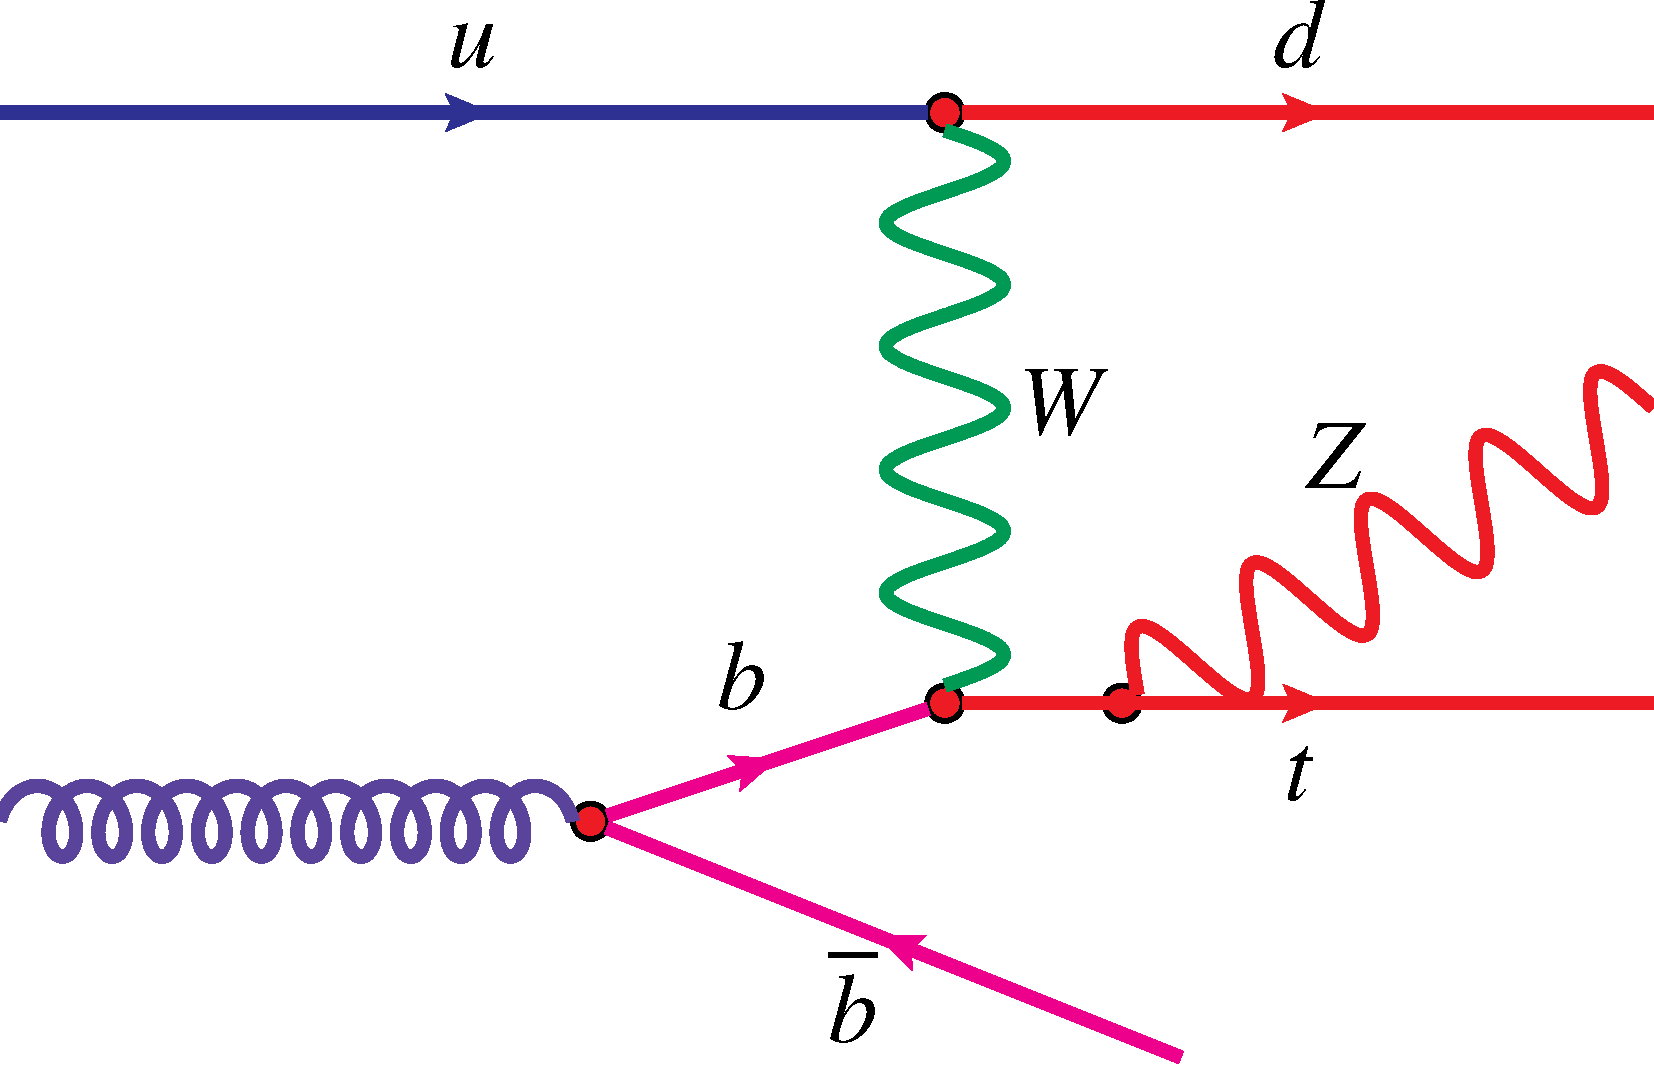
\includegraphics[width=0.4\textwidth]{../pyfeyn/tZq_4FS_feyn}
  }
  \quad
  \raisebox{2ex}{%
    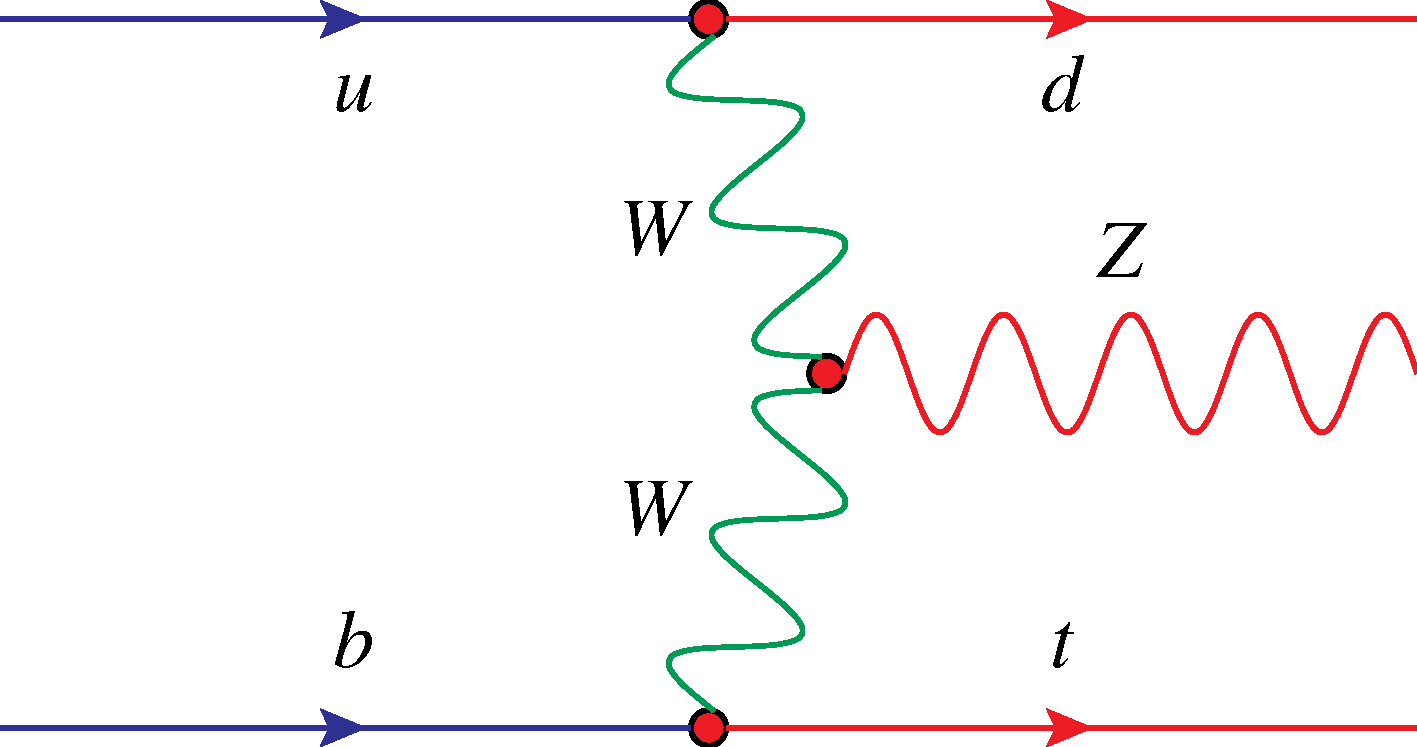
\includegraphics[width=0.4\textwidth]{../pyfeyn/tZq_5FS_feyn}
  }
  \caption{Example Feynman graphs for the associated production
    of a top quark and a \PZ boson.}%
  \label{fig:tZq-pyfeyn}
\end{figure}


%------------------------------------------------------------------------------
\subsection{FeynMP}%
\label{sec:fig:feynman:feynmp}\index{feynmp}

In order to use the \Package{feynmp} package, you have to put
the commands to draw the graph in a \LaTeX{} file and then process
this file with \LaTeX{} and either Metafont or
Metapost.\footnote{\texttt{ubonn-thesis.sty} now includes \Package{feynmp}
  by default for \TeXLive 2011 and later. If you want to use
  \Package{feynmf} instead just change the name.} 
You can either make
a separate \LaTeX{} file containing the Feynman graph or include the
commands inside your normal \LaTeX\ file.
Metapost\index{metapost} is a bit easier to use than Metafont.
You should be able to just run
\texttt{mpost} after \texttt{(pdf)latex} and then run % chktex 36
\texttt{pdflatex} again twice.
Note that you have to run
\texttt{mpost} on all the files whose names are defined at the
beginning of the \Env{fmffile} environment.\footnote{%
  While Metapost works well
  as of \TeXLive 2011, I did not get it to work properly with \TeXLive
  2009 for unknown reasons.}

Metafont\index{metafont} is a bit trickier and details have been relegated to
\cref{sec:app:fig:feynman:feynmf}. 
On Unix systems the \texttt{feynmf} perl script exists that runs both \LaTeX{} and
Metafont for you. This will produce a \texttt{dvi} file that you then
then look at or use to make a Postscript/PDF file.

I think a better way to proceed is the following:
\begin{itemize}
\item make a separate \LaTeX{} file for each of the Feynman graphs;
\item input this file in your figure;
\item use the \File{Makefile} described below to automatically run
  over one or all \Package{feynmp}/\Package{feynmf} \LaTeX{} files by giving the
  command \texttt{make feynmp} or \texttt{make feynmf}.\\
  Check
  \texttt{./feynmf/feynmf\_all.dvi} or
  \texttt{./feynmf/feynmf\_all.pdf} to see if the graphs are OK\@;
\item run \LaTeX{} or pdf\LaTeX; % chktex 13
\item run \texttt{bibtex} or \texttt{biber};
\item run \LaTeX{} or pdf\LaTeX{} again, at least twice.
\end{itemize}
The last three steps are done with the command \texttt{make thesis},
\texttt{make thesis11} or
\texttt{make thesis09}.
The big advantage of this procedure is that the graphs are included
\enquote{properly} in the thesis, their fonts should automatically
match the fonts used in the thesis and you don't have to worry about
converting and clipping. I have written a small script that is
executed by the \texttt{Makefile} to do the third step.
The script is \texttt{run\_mf} for \Package{feynmf} and
\texttt{run\_mp} for \Package{feynmp}. These are
included in the main directory \File{ubonn-thesis}.
The scripts assume that all Feynman graphs are in 
a \texttt{feynmf} subdirectory. This can clearly be
adjusted in the \texttt{Makefile} as necessary.
To get started you can copy the \File{feynmf} directory from \File{ubonn-thesis}.

The \texttt{run\_mf} script assumes that all files of type
\texttt{tex} (except those that start with \texttt{feynmf\_}) are
Feynman graphs to process with \texttt{feynmf}. Note that it may be
necessary to give the command \texttt{make cleanfeynmf} to get rid of
temporary files before \texttt{make feynmf} if you change the sizes of
things.

The \texttt{run\_mp} script works a bit differently. It creates a
temporary directory \texttt{mpost\_tmp} in which it processes the
figures (\texttt{tex} files) in the \texttt{feynmf} subdirectory. The
resulting PDF files are copied back to the \texttt{feynmf}
subdirectory.

You can also use the package \Package{standalone} together with
\Package{feynmp}. The files in the \texttt{feynmf} directory contain
commented out code that shows how this can be done. I do not do this
by default for the guide, as the package is very new and I also want
to test making the Feynman graphs with \Package{feynmf}. Note that
the name in the \Env{fmffile} environment (and the \Macro{write18}
command) should be the same and different from the name of the \LaTeX\
file. If you use this option, you should probably also adjust the
\texttt{Makefile} target for \texttt{feynmp} to work in the same way
as the target \texttt{tikz}. You have to run \texttt{pdflatex} twice
on each file.

\Cref{fig:nccc-feynmf} shows the same neutral current and
charged current graphs, but this time inputting the appropriate
\Package{feynmf} commands directly. The graphs are enclosed in
\Macro{fbox} for illustration purposes only.
The plots are made using \Package{feynmp},
where an appropriate
\Macro{write18} statement is included in the \LaTeX\ source code,
e.g.\ \verb+\write18 mpost gluon+, after the figure, where the figure
starts with \verb+\begin{fmffile}{gluon}+.%
\footnote{If you use \TeXstudio you may have to give the full pathname for \texttt{mpost},
  e.g.\ \texttt{/usr/texbin/mpost}, as \TeXstudio does not parse your \texttt{PATH} properly.}

\begin{figure}[htbp]
  \centering
  \fbox{%
% Electron-proton NC scattering
%
% Comment in the lines from \documentclass to \begin{document}
% and from \write18 to \end{document}
% to use the standalone package for testing the Feynman graphs
% You should also change the fmffile name to ep_cc-mp
% \documentclass{standalone}

% \usepackage{feynmp}
% \DeclareGraphicsRule{*}{mps}{*}{}

% \unitlength=1mm
% \begin{document}
\begin{fmffile}{ep_nc}
\begin{fmfgraph*}(50,50) \fmfpen{thin}
  \fmfleft{i1,i2} \fmfright{o1,o2}
  \fmfv{label=$X$,l.angle=10,l.dist=3*thick}{o1}
  \fmf{heavy,label=$p(P)$,l.side=left}{i1,v1}
  \fmf{plain}{v1,o1}
  \fmf{fermion,lab=$e(k)$,l.side=right}{i2,v2}
  \fmf{fermion,lab=$e^\prime(k^\prime)$}{v2,o2}
  \fmf{photon,lab=$\gamma,, Z(q)$,l.side=right}{v1,v2}
  \fmfv{decor.shape=circle,decor.filled=.5,decor.size=.20w}{v1}
  \fmfdot{v2}
  \fmffreeze
  \fmfi{plain}{vpath (__v1,__o1) shifted (thick*(0.7,2))}
  \fmfi{plain}{vpath (__v1,__o1) shifted (thick*(-1,-2))}
\end{fmfgraph*}
\end{fmffile}
% Include this command for Metapost
% \write18{mpost ep_nc-mp}
% \end{document}
}
  % \ifthenelse {\texlive < 2011} {%
  % }{
    \write18{mpost ep_nc}
  % }
  \qquad
  \fbox{%
% Electron-proton CC scattering
%
\begin{fmffile}{ep_cc}
\begin{fmfgraph*}(50,50) \fmfpen{thin}
  \fmfleft{i1,i2} \fmfright{o1,o2}
  \fmfv{label=$X$,l.angle=10,l.dist=3*thick}{o1}
  \fmf{heavy,label=$p(P)$,l.side=left}{i1,v1}
  \fmf{plain}{v1,o1}
  \fmf{fermion,lab=$e(k)$,l.side=right}{i2,v2}
  \fmf{fermion,lab=$\nu_{e}(k^\prime)$}{v2,o2}
  \fmf{dashes,lab=$W^{\pm}(q)$,l.side=right}{v1,v2}
  \fmfv{decor.shape=circle,decor.filled=.5,decor.size=.20w}{v1}
  \fmfdot{v2}
  \fmffreeze
  \fmfi{plain}{vpath (__v1,__o1) shifted (thick*(0.7,2))}
  \fmfi{plain}{vpath (__v1,__o1) shifted (thick*(-1,-2))}
\end{fmfgraph*}
\end{fmffile}
}
  % \ifthenelse {\texlive < 2011} {%
  % }{
    \write18{mpost ep_cc}
  % }
  \caption{NC and CC graphs for $ep$ scattering using \Package{feynmf}
    code directly.}%
  \label{fig:nccc-feynmf}
\end{figure}

With the \TeXLive 2011 and later setups I use to test this guide,
this is all you need. If \texttt{mpost} does not run automatically,
you must execute the command
\texttt{pdflatex --shell-escape mythesis} when you compile your thesis.
This can be achieved by
including the \texttt{EXTRACMD} definition that is commented out in
the \texttt{Makefile}.
In this guide I put the Feynman graph in its
own file and the \Macro{write18} statement in the main file so that
I can test \Package{feynmf} and \Package{feynmp} with the same
\LaTeX\ code. In your thesis, you should probably put the
\Macro{write18} statement in the file with the Feynman graph.
If you use \Command{latexmk}\index{latexmk} to compile you probably need to use 
the commented out version of the \Command{latexmk} command in the \File{Makefile}.

As mentioned above, you probably want to first draw the graphs outside
of your thesis to get them into the form that you need. If you give
the command \texttt{make feynmf}, it will run \texttt{feynmf} on all
\texttt{tex} files in the subdirectory \texttt{feynmf}. If you give
the command \texttt{make feynmf file=ep\_nc} it will run over
\texttt{./feynmf/ep\_nc.tex} etc. As indicated above, the graphs can
then be looked at in \texttt{feynmf\_all.dvi} or\\
\texttt{feynmf\_all.pdf}. You can use the same syntax for
\texttt{make feynmp} and \texttt{make tikz}.


%------------------------------------------------------------------------------
\section{\TikZ and PGF}%
\label{sec:fig:tikz}\index{TikZ@\TikZ}
%------------------------------------------------------------------------------

\Package{pgfplots} and \Package{\TikZ} are packages to help with
creating graphics \enquote{inline}.
For 3D figures you also need \Package{tikz-3dplot}.
PGF is the backend, while \TikZ is what the user interacts with directly.
The manual contains all the information you should need,
but was 1318 pages long at the last count,
so it may not to be too easy to find what you want!

I do not have much experience with using these packages so far,
except for Feynman graphs discussed above.
Hence, this section will certainly not cover all possibilities. There may
also be better ways of doing things than I illustrate here. The
examples I give come from Andrii Verbytskyi or are adapted from
questions and answers found on
\url{http://tex.stackexchange.com/}.
The examples included in this
guide and a few more are collected in the \texttt{tikz} directory.
If you want to get started with \TikZ you can copy this directory
into your thesis directory, e.g.\ \File{mythesis}.
% \footnote{%
% Note that some of the examples only work with \TeXLive
% 2011 and later. This is indicated in the file.
% I also did not manage
% to compile the guide without errors when including \Package{\TikZ} with
% \TeXLive 2009, so some of the figures may be missing if you compile
% your own version of the guide with \TeXLive 2009.}

\TikZ is not included by default in a new skeleton thesis. See the
commented out packages in a new thesis skeleton or
\texttt{thesis\_guide.tex} for the packages and \TikZ libraries that
you should include if you want to use it.

You often want to include a figure of your experiment's coordinate
system in your thesis. One way to do this is illustrated in
\cref{fig:tikz:coord}.

\begin{figure}[htbp]
  \centering
  % The ZEUS coordinate system
\setstretch{1.0}
\tdplotsetmaincoords{60}{160}
\begin{tikzpicture}[tdplot_main_coords]
  \draw[thick,->] (-1,0,0) -- (3,0,0) node[anchor=north east]{$z$};
  \draw[thick,->] (0,0,0)  -- (0,4,0) node[anchor=north west]{$x$};
  \draw[thick,->] (0,0,0)  -- (0,0,4) node[anchor=south]{$y$};
  \tdplotdefinepoints(0,0,0)(5,0,0)(3,3,3)
  \draw[dashed,black]  (\tdplotbx,\tdplotby,\tdplotbz) -- (\tdplotvertexx,\tdplotvertexy,\tdplotvertexz);
  \tdplotdrawpolytopearc[thick]{1}{anchor=east}{$\theta$}
  \tdplotdefinepoints(0,0,0)(0,5,0)(0,5,5)
  \draw[dashed,black]  (\tdplotbx,\tdplotby,\tdplotbz) -- (\tdplotvertexx,\tdplotvertexy,\tdplotvertexz);
  \tdplotdrawpolytopearc[thick]{1}{anchor=west}{$\phi$}
  \draw[->,thick,red]  (0,0,0)  -- (3,3,3);
  \draw[black,dashed]  (3,3,3)  -- (0,3,3);
  \draw[blue,thick,->] (6,0,0)  -- (4,0,0)  node[anchor=south east]{$e$};
  \draw[blue,thick,->] (-4,0,0) -- (-2,0,0) node[anchor=south west]{$p$};
\end{tikzpicture}

    % \ifthenelse {\texlive < 2012} {%
  %   \fbox{\parbox[c]{0.8\textwidth}{%
  %   Sorry, \Package{tikz-3dplots} is not available in \TeXLive 2009 and
  %   earlier. See the file \texttt{./tikz/zeus\_coords.tex}.}
  %   This example also does not work with \TeXLive 2011.}
  % }{%
  %   % The ZEUS coordinate system
\setstretch{1.0}
\tdplotsetmaincoords{60}{160}
\begin{tikzpicture}[tdplot_main_coords]
  \draw[thick,->] (-1,0,0) -- (3,0,0) node[anchor=north east]{$z$};
  \draw[thick,->] (0,0,0)  -- (0,4,0) node[anchor=north west]{$x$};
  \draw[thick,->] (0,0,0)  -- (0,0,4) node[anchor=south]{$y$};
  \tdplotdefinepoints(0,0,0)(5,0,0)(3,3,3)
  \draw[dashed,black]  (\tdplotbx,\tdplotby,\tdplotbz) -- (\tdplotvertexx,\tdplotvertexy,\tdplotvertexz);
  \tdplotdrawpolytopearc[thick]{1}{anchor=east}{$\theta$}
  \tdplotdefinepoints(0,0,0)(0,5,0)(0,5,5)
  \draw[dashed,black]  (\tdplotbx,\tdplotby,\tdplotbz) -- (\tdplotvertexx,\tdplotvertexy,\tdplotvertexz);
  \tdplotdrawpolytopearc[thick]{1}{anchor=west}{$\phi$}
  \draw[->,thick,red]  (0,0,0)  -- (3,3,3);
  \draw[black,dashed]  (3,3,3)  -- (0,3,3);
  \draw[blue,thick,->] (6,0,0)  -- (4,0,0)  node[anchor=south east]{$e$};
  \draw[blue,thick,->] (-4,0,0) -- (-2,0,0) node[anchor=south west]{$p$};
\end{tikzpicture}

  % }
  \caption{The ZEUS coordinate system.}%
  \label{fig:tikz:coord}
\end{figure}

It is also possible to make flow charts with \TikZ.
This is illustrated in \cref{fig:tikz:flow}.

\begin{figure}[htbp]
  \centering
  \documentclass{standalone}

\usepackage{siunitx}
\usepackage{tikz}
\usepackage{tikz-3dplot}
\usepackage{pgfplots}
\usetikzlibrary{positioning,shapes,arrows}
\usetikzlibrary{decorations.pathmorphing}
\usetikzlibrary{decorations.markings}

\begin{document}
% \setstretch{1.0}
\tikzstyle{decision} = [diamond, draw, fill=blue!20,
    text width=4.5em, text badly centered, node distance=3cm, inner sep=0pt]
\tikzstyle{block} = [rectangle, draw, fill=blue!20,
    text width=5em, text centered, rounded corners, minimum height=4em]
\tikzstyle{block2} = [rectangle, draw, fill=blue!20,
    text width=5em, text centered, rounded corners, minimum height=4em, minimum width=10em]
\tikzstyle{line} = [draw, -latex']
\tikzstyle{cloud} = [draw, ellipse,fill=red!20, node distance=3cm,
minimum height=2em]
\begin{tikzpicture}
  [scale=1.68]
  \clip (-6.0cm,0.6cm) rectangle (2.6cm,-9.6cm);
  \node[draw,    ellipse,fill=red!20,   text centered,minimum height=16mm, text width=24mm](Generator) at (-1cm,0mm){Event generator};
  \node[draw,    ellipse,fill=red!20,   text centered,minimum height=16mm, text width=24mm](Collision) at (0.8cm,0mm){Collision};
  \node[rectangle, draw, fill=blue!20,  text width=22mm, minimum height=12mm, text centered, rounded corners](MOZART)    at (-1cm,-1.5cm){MOZART};
  \node[rectangle, draw, fill=blue!20,  text width=22mm, minimum height=12mm, text centered, rounded corners](Detector)  at (0.8cm, -1.5cm){Detector};
  \node[rectangle, draw, fill=blue!20,  text width=22mm, minimum height=12mm, text centered, rounded corners](ZGANA)     at (-1cm,-3.0cm){ZGANA};
  \node[rectangle, draw, fill=blue!20,  text width=22mm, minimum height=12mm, text centered, rounded corners](Trigger)   at (0.8cm, -3.0cm){Trigger};
  \node[rectangle, draw, fill=white!20, text width=22mm, minimum height=12mm, text centered, rounded corners](Rejection) at (1.8cm, -4.5cm){Event rejection};
  \node[rectangle, draw, fill=blue!20,  text width=22mm, minimum height=12mm, text centered, rounded corners](ZEPHYR)    at (-0.1cm, -4.5cm){ZEPHYR};
  \node[rectangle, draw, fill=blue!20,  text width=22mm, minimum height=12mm, text centered, rounded corners](Orange)    at (-0.1cm, -6.0cm){ORANGE and PHANTOM};
  \node[rectangle, draw, fill=white!20, text width=22mm, minimum height=12mm, text centered, rounded corners](NTP)       at (-0.1cm, -7.5cm){NTuples};
  \node[rectangle, draw, fill=white!20, text width=22mm, minimum height=12mm, text centered, rounded corners](AN)        at (-0.1cm, -9.0cm){Analysis};


  \node [draw, ellipse,fill=red!20,    minimum height=3mm,  text centered, text width=45.0mm]  (MCC)   at (-4cm,-1.15cm) {MOZART control cards};
  \node [draw, ellipse,fill=red!20,    minimum height=3mm,  text centered, text width=45.0mm]  (MGF)   at (-4cm,-1.65cm) {MOZART GAFs};

  \node [draw, ellipse,fill=red!20,    minimum height=3mm,  text centered, text width=45.0mm]  (ZCC)   at (-4cm,-2.65cm) {ZGANA control cards};
  \node [draw, ellipse,fill=red!20,    minimum height=3mm,  text centered, text width=45.0mm]  (ZGF)   at (-4cm,-3.15cm) {ZGANA GAFs};


  \node [draw, ellipse,fill=red!20,    minimum height=3mm,  text centered, text width=45.0mm]  (ZPCC)  at (-4cm,-4.15cm) {ZEPHYR control cards};
  \node [draw, ellipse,fill=red!20,    minimum height=3mm,  text centered, text width=45.0mm]  (ZPGF)  at (-4cm,-4.65cm) {ZEPHYR GAFs};

  \node [draw, ellipse,fill=red!20,    minimum height=3mm,  text centered, text width=45.0mm]  (OCC)   at (-4cm,-5.65cm) {ORANGE control cards};
  \node [draw, ellipse,fill=red!20,    minimum height=3mm,  text centered, text width=45.0mm]  (OGF)   at (-4cm,-6.15cm) {ORANGE GAFs};


  \path [line,dashed] (Generator) -- (MOZART);
  \path [line,dashed] (Collision) -- (Detector);


  \path [line,dashed] (MCC) -- (MOZART);
  \path [line,dashed] (MGF) -- (MOZART);


  \path [line,dashed] (ZCC) -- (ZGANA);
  \path [line,dashed] (ZGF) -- (ZGANA);

  \path [line,dashed] (ZPCC) -- (ZEPHYR);
  \path [line,dashed] (ZPGF) -- (ZEPHYR);

  \path [line,dashed] (OCC) -- (Orange);
  \path [line,dashed] (OGF) -- (Orange);


  \path [line] (MOZART) -- (ZGANA);
  \path [line]  (ZGANA) -- (ZEPHYR);

  \path [line] (Detector) -- (Trigger);
  \path [line]  (Trigger) -- (ZEPHYR);
  \path [line]  (Trigger) -- (Rejection);

  \path [line]  (ZEPHYR) -- (Orange);
  \path [line]  (Orange) -- (NTP);
  \path [line]  (NTP) -- (AN);
\end{tikzpicture}
\end{document}

  % \ifthenelse {\texlive < 2011} {%
  %   \fbox{\parbox[c]{0.8\textwidth}{%
  %       Error messages appear when trying to compile the guide with
  %       \Package{tikz} and \TeXLive 2009, so the figure is not included.
  %       See the file \texttt{../tikz/zeus\_reconstruction.tex}.}}
  % }{%
  %   \documentclass{standalone}

\usepackage{siunitx}
\usepackage{tikz}
\usepackage{tikz-3dplot}
\usepackage{pgfplots}
\usetikzlibrary{positioning,shapes,arrows}
\usetikzlibrary{decorations.pathmorphing}
\usetikzlibrary{decorations.markings}

\begin{document}
% \setstretch{1.0}
\tikzstyle{decision} = [diamond, draw, fill=blue!20,
    text width=4.5em, text badly centered, node distance=3cm, inner sep=0pt]
\tikzstyle{block} = [rectangle, draw, fill=blue!20,
    text width=5em, text centered, rounded corners, minimum height=4em]
\tikzstyle{block2} = [rectangle, draw, fill=blue!20,
    text width=5em, text centered, rounded corners, minimum height=4em, minimum width=10em]
\tikzstyle{line} = [draw, -latex']
\tikzstyle{cloud} = [draw, ellipse,fill=red!20, node distance=3cm,
minimum height=2em]
\begin{tikzpicture}
  [scale=1.68]
  \clip (-6.0cm,0.6cm) rectangle (2.6cm,-9.6cm);
  \node[draw,    ellipse,fill=red!20,   text centered,minimum height=16mm, text width=24mm](Generator) at (-1cm,0mm){Event generator};
  \node[draw,    ellipse,fill=red!20,   text centered,minimum height=16mm, text width=24mm](Collision) at (0.8cm,0mm){Collision};
  \node[rectangle, draw, fill=blue!20,  text width=22mm, minimum height=12mm, text centered, rounded corners](MOZART)    at (-1cm,-1.5cm){MOZART};
  \node[rectangle, draw, fill=blue!20,  text width=22mm, minimum height=12mm, text centered, rounded corners](Detector)  at (0.8cm, -1.5cm){Detector};
  \node[rectangle, draw, fill=blue!20,  text width=22mm, minimum height=12mm, text centered, rounded corners](ZGANA)     at (-1cm,-3.0cm){ZGANA};
  \node[rectangle, draw, fill=blue!20,  text width=22mm, minimum height=12mm, text centered, rounded corners](Trigger)   at (0.8cm, -3.0cm){Trigger};
  \node[rectangle, draw, fill=white!20, text width=22mm, minimum height=12mm, text centered, rounded corners](Rejection) at (1.8cm, -4.5cm){Event rejection};
  \node[rectangle, draw, fill=blue!20,  text width=22mm, minimum height=12mm, text centered, rounded corners](ZEPHYR)    at (-0.1cm, -4.5cm){ZEPHYR};
  \node[rectangle, draw, fill=blue!20,  text width=22mm, minimum height=12mm, text centered, rounded corners](Orange)    at (-0.1cm, -6.0cm){ORANGE and PHANTOM};
  \node[rectangle, draw, fill=white!20, text width=22mm, minimum height=12mm, text centered, rounded corners](NTP)       at (-0.1cm, -7.5cm){NTuples};
  \node[rectangle, draw, fill=white!20, text width=22mm, minimum height=12mm, text centered, rounded corners](AN)        at (-0.1cm, -9.0cm){Analysis};


  \node [draw, ellipse,fill=red!20,    minimum height=3mm,  text centered, text width=45.0mm]  (MCC)   at (-4cm,-1.15cm) {MOZART control cards};
  \node [draw, ellipse,fill=red!20,    minimum height=3mm,  text centered, text width=45.0mm]  (MGF)   at (-4cm,-1.65cm) {MOZART GAFs};

  \node [draw, ellipse,fill=red!20,    minimum height=3mm,  text centered, text width=45.0mm]  (ZCC)   at (-4cm,-2.65cm) {ZGANA control cards};
  \node [draw, ellipse,fill=red!20,    minimum height=3mm,  text centered, text width=45.0mm]  (ZGF)   at (-4cm,-3.15cm) {ZGANA GAFs};


  \node [draw, ellipse,fill=red!20,    minimum height=3mm,  text centered, text width=45.0mm]  (ZPCC)  at (-4cm,-4.15cm) {ZEPHYR control cards};
  \node [draw, ellipse,fill=red!20,    minimum height=3mm,  text centered, text width=45.0mm]  (ZPGF)  at (-4cm,-4.65cm) {ZEPHYR GAFs};

  \node [draw, ellipse,fill=red!20,    minimum height=3mm,  text centered, text width=45.0mm]  (OCC)   at (-4cm,-5.65cm) {ORANGE control cards};
  \node [draw, ellipse,fill=red!20,    minimum height=3mm,  text centered, text width=45.0mm]  (OGF)   at (-4cm,-6.15cm) {ORANGE GAFs};


  \path [line,dashed] (Generator) -- (MOZART);
  \path [line,dashed] (Collision) -- (Detector);


  \path [line,dashed] (MCC) -- (MOZART);
  \path [line,dashed] (MGF) -- (MOZART);


  \path [line,dashed] (ZCC) -- (ZGANA);
  \path [line,dashed] (ZGF) -- (ZGANA);

  \path [line,dashed] (ZPCC) -- (ZEPHYR);
  \path [line,dashed] (ZPGF) -- (ZEPHYR);

  \path [line,dashed] (OCC) -- (Orange);
  \path [line,dashed] (OGF) -- (Orange);


  \path [line] (MOZART) -- (ZGANA);
  \path [line]  (ZGANA) -- (ZEPHYR);

  \path [line] (Detector) -- (Trigger);
  \path [line]  (Trigger) -- (ZEPHYR);
  \path [line]  (Trigger) -- (Rejection);

  \path [line]  (ZEPHYR) -- (Orange);
  \path [line]  (Orange) -- (NTP);
  \path [line]  (NTP) -- (AN);
\end{tikzpicture}
\end{document}

  % }
  \caption[Event reconstruction and simulation in ZEUS]{Event reconstruction and simulation in ZEUS.}%
  \label{fig:tikz:flow}
\end{figure}

There are many more possibilities,
including plots which you would otherwise make with \texttt{root} or
some other graphics program. An example plot showing the effect of
systematic variations can be found in \cref{sec:app:tikz}. Making
Feynman graphs with \TikZ is covered in \cref{sec:fig:feynman:tikz}.


%------------------------------------------------------------------------------
\subsection{Accelerator lattices}%
\label{sec:fig:accelerator}

If you want to include an accelerator lattice in your thesis you can try
\Package{tikz-palattice}\footnote{%
  \url{https://ctan.org/pkg/tikz-palattice}
written by Jan Schmidt, who gave me a number of useful tips for this guide.}
He used the package to make lattices of particle accelerators for his PhD thesis.

